\documentclass{article}

\usepackage[T1]{fontenc}
\usepackage{cite}
\usepackage{graphicx} 
\usepackage{caption}    
\usepackage{subcaption} 
\usepackage{booktabs}
\usepackage{array}

\renewcommand{\arraystretch}{1.2}
\setlength{\tabcolsep}{6pt}

\title{Capacitively-Coupled Chopper Instrumentation Amplifier for Linear Hall Effect Sensor \\[1ex] \large IEEE SSCS Chipathon 2026}
\author{Team Chop}
\date{\today}

\begin{document}

\maketitle

\newpage

\section{Introduction}

\cite{Lamport1994}

\begin{itemize}
    \item Discuss magnetic sensing application space
        \begin{itemize}
            \item Current sensing
            \item Tactile Sensing (robotics)
            \item Position/Velocity Sensing (automotive)
            \item Biosensors
        \end{itemize}
    \item Discuss utility of building open-source Hall sensor readout
        \begin{itemize}
            \item No existing data on n-well-based Hall sensors in open PDKs
            \item Sensor evaluation gives future designers ability to integrate into their application
            \item Readout circuit directly applicable to most bridge-type sensors
        \end{itemize}
\end{itemize}

\newpage

\section{Conceptual Design}

\begin{itemize}
    \item Show high-level block diagram
    \item Table of pinouts with signal descriptions/directions
\end{itemize}

\begin{figure}[htbp]
    \centering
    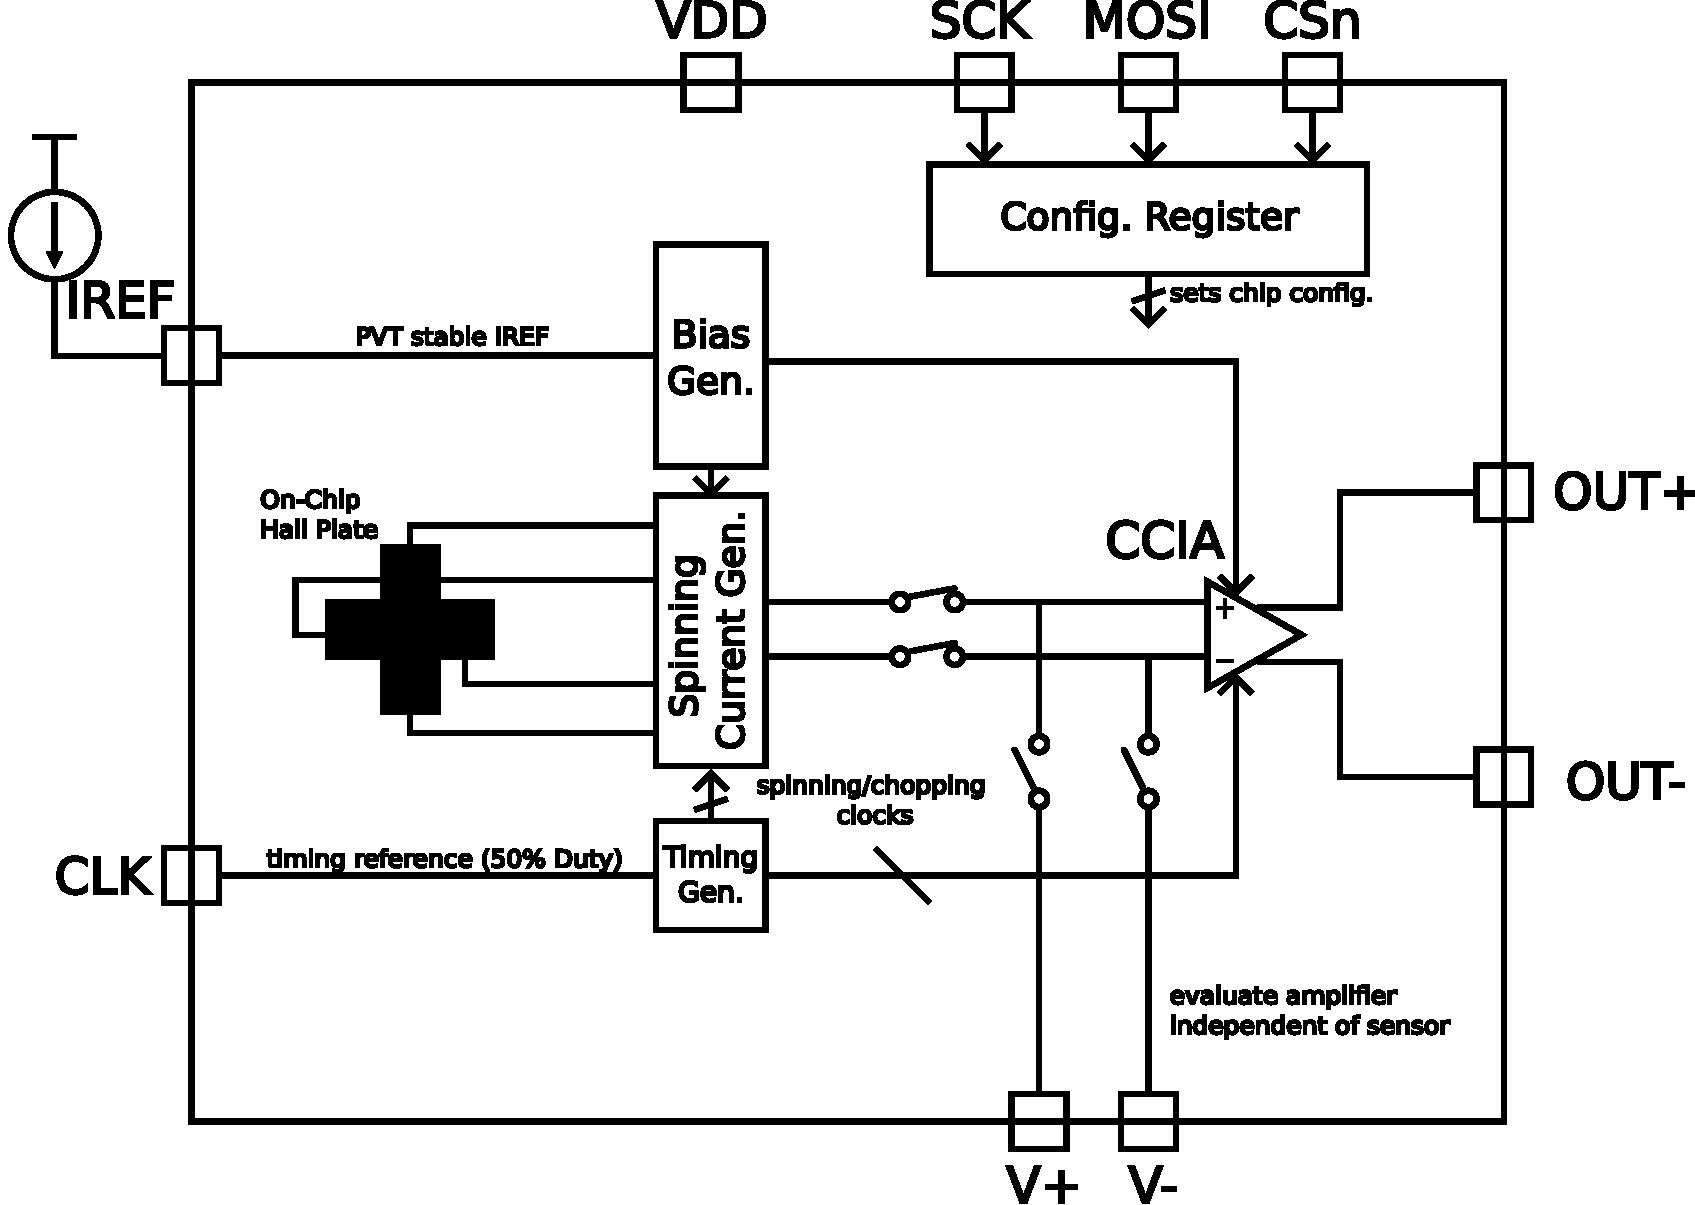
\includegraphics[width=0.8\linewidth]{figs/chip_block_diagram.pdf}
    \caption{Block diagram of the proposed architecture.}
    \label{fig:block_diagram}
\end{figure}

Fig.~\ref{fig:block_diagram}

\begin{table}[htbp]
\centering
\caption{Chip pinout description.}
\label{tab:pinout}

\begin{tabular}{p{2.2cm} p{2.5cm} p{8.0cm}}
\toprule

\multicolumn{3}{l}{\textbf{Analog Pins}} \\
\midrule
IREF   & Analog & Current reference \\
OUT+   & Analog & Differential output positive terminal \\
OUT-   & Analog & Differential output negative terminal \\
VTP+   & Analog & Positive analog test point (differential probe node) \\
VTP-   & Analog & Negative analog test point (differential probe node) \\
\midrule

\multicolumn{3}{l}{\textbf{Digital Interface}} \\
\midrule
SCK    & Digital Input & SPI configuration clock \\
MOSI   & Digital Input & SPI configuration data input \\
CSn    & Digital Input & SPI chip select (active low; data shifted while low, latched on rising edge) \\
CLK    & Digital Input & Chopping/spinning clock reference \\
\midrule

\multicolumn{3}{l}{\textbf{Supply Pins}} \\
\midrule
VDD    & Power & Supply input \\
VSS    & Power & Ground (shared with other Chipathon blocks) \\
\bottomrule

\end{tabular}
\end{table}

Table~\ref{tab:pinout}

\subsection{Sensor}

\begin{itemize}
    \item Vertical vs. Horizontal sensor design
    \item Horizontal sensor geometries
    \item 
\end{itemize}

\subsection{Readout Circuit}

\begin{itemize}
    \item Instrumentation Amplifier options/survey
    \item CCIA chosen due to large common-mode input range (sweepable bias current), stable gain (easy to integrate several gain options if needed)
    \item Hall sensor bias expected to dominate power consumption, but CCIA being low-power is great in other high-impedance sensor applications
    \item analog output reduces complexity and allows for easier characterization of CCIA
\end{itemize}

\newpage

\section{Design Specifications}

\begin{itemize}
    \item Table of specifications for full system
\end{itemize}

\subsection{Sensor}

\subsection{Readout Circuit}

\newpage

\section{Schematic Design}

\begin{itemize}
    \item Show top-level schematic 
\end{itemize}

\subsection{Subblock 1}

\subsection{Subblock N}

\newpage

\section{Layout Design}

\begin{itemize}
    \item Show layout floorplan
\end{itemize}

\subsection{Subblock 1}

\subsection{Subblock N}

\newpage

\section{Simulation Results}

\begin{itemize}
    \item Verification Plan details (how is each specification tested?)
\end{itemize}

\subsection{Simulation 1}

\subsection{Simulation M}

\newpage

\bibliographystyle{IEEEtran}
\bibliography{references}

\end{document}